\documentclass[]{article}
\usepackage[justification=centering]{caption}
\usepackage{csvsimple}
\usepackage{tabulary}
\usepackage{graphicx}
\usepackage{float}
\graphicspath{{../img/}}

\newcommand{\getMeasuredC}{$C = 0.454 \mu F \pm 0.002 \mu F $}
\newcommand{\getMeasuredR}{$R_{L} = 26.7 \Omega \pm 0.1 \Omega $}
\newcommand{\getFrequency}{$f = 1000 Hz$}


\title{ENPHYS253 \\ Lab 3: Electrical Impedance}
\author{Viraj Bangari \\ 10186046}
\date{\today}

\begin{document} 
\maketitle

\begin{abstract}
    The impedances of an inductor and capacitor at 1000 Hz were experimentally
    determined by measuring the RMS values of the components in various circuit
    configuration with a digital multimeter. AC circuits with either one
    inductor or capacitor were constructed with varying input voltage
    frequencies. The RMS current and voltage values were used to create a series
    of linear regressions which determined that $R_L = 27.7 \Omega \pm 5 *
    10^{-2} \Omega$, $L = 1.12 * 10 ^{-2} H \pm 9 * 10^{-6} H$ and $R_C = 24
    \Omega \pm 6 \Omega$, $C = 4.56*10^{-7} F \pm 3*10^{-10} F$. A parallel and
    series LC circuit was created at 1000Hz with varying input voltage frequency
    from the function generator. By finding a linear relationship between
    $I_{rms}$ and $V_{rms}$ through linear regression, an impedance value was
    determined. The capacitance and inductance were used with theoretical
    equations for impedance and to compare with experimentally derived
    impedance. All the predictions from the theoretical impedances were within
    error of the physically measured impedance, verifying that the impedance
    values at 1000Hz were $Z_L = 27.7 \Omega + 70.5j \Omega$  and $Z_C = -349j
    \Omega$.
\end{abstract}

\section*{Results and Analysis}
The voltage and current data for the single inductor with \getMeasuredR\ circuit
from Table~\ref{tab:ind} was graphed according to Equation~\ref{eq2} onto
Figure~\ref{fig:ind}. A weighted linear regression was performed, giving a
result of $R_L = 27.7 \Omega \pm 5 * 10^{-2} \Omega$ and $L = 1.12 * 10 ^{-2}
H \pm 9 * 10^{-6} H$. The derived value for $R_L$ agrees with the $26.7 \Omega \pm
0.1 \Omega$ reading obtained by using a multimeter on the inductor as it lies
within the error range and has a percentage difference of 3.8\% Using the
data in Table~\ref{tab:cap} with Equation~\ref{eq3} where a single capacitor
circuit with \getMeasuredC\ was used, a weighted linear regression was created
onto Figure~\ref{fig:cap}. The regression gave that $R_C = 24 \Omega \pm
6 \Omega$ and $C = 4.56*10^{-7} F \pm 3*10^{-10} F$. The value of $C$ agrees with
the value of the measurement \getMeasuredC\ obtained from the multimeter as the
values lie within their margins of error and have a percentage difference of
0.47\%.

Using Equation 2, the $V_{rms}$ and $I_{rms}$ values in Table 3 measured from
the Parallel LC circuit were plotted against each other in Figure 3, and a
linear regression was used to determine that $|Z_{Parallel}| = 95.3 \Omega \pm
0.3 \Omega$. Similarly, the values from the series LC on Table 4 were plotted
with linear regression to determine that $|Z_{series}| = 284 \Omega \pm 1
\Omega$. Using the test frequency of $1000 Hz$ and equations 5 and 6 with the
$R_L, L$ and $C$ values obtained earlier, the impedances were determined to be
$Z_L = 27.7 + 70.5j \Omega$ and $Z_C = -349j \Omega$. Using equations 7 and 9 to
combine the impedances in parallel and series, $|Z_{Parallel}'|$ and
$|Z_{Series}'|$ values were determined as $94.5 \Omega \pm 0.9 $ and $280 \Omega
\pm 2 \Omega$.  These values lie within the range of the expected values, and
have percentage difference of only 0.9\% and 1.42\%.

The values of $|Z_{Parallel}'|$ and  $|Z_{Series}'|$ were verified by using them
with Equation 2 to predict an expected $V_{rms}$ and $I_{rms}$ by comparing it
to a measured value. The $I_L$ and $I_C$ values were physically measured at max
voltage in the parallel LC circuit on Table 3 as $I_L = 77.2 mA \pm 0.37 mA$ and
$I_C = 16.8 mA \pm 0.84 mA $. Using Equation 2 with $Z_L$ and $Z_C$, the
expected values are $I_C = 77.3 mA \pm 0.3 mA$ and $I_L = 16.8 mA \pm 0.4 mA$
values within the range of the measured values, having a percentage difference
of 0.03\% and 0\% respectively. In the series LC circuit, the $V_{rms}$ values
were measured as $V_L = 1.89 V \pm 0.94 V$ and $V_C = 9.36 V \pm 0.47 V$ on
Table 4.  Using Equation 2, the expected values values are $V_L = 2.02 \pm 0.07$
and $V_C = 9.31 \pm 0.04$. The Voltage values all lie within the range of
uncertainty and have a respective percentage difference of 7.0\% and 0.47\%

\newpage
\begin{figure}[H]
    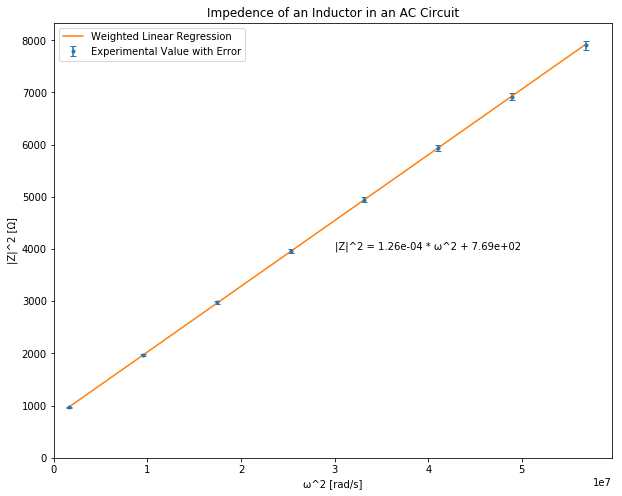
\includegraphics[width=\textwidth]{ind.png}
    \caption{Impedance of an Inductor in an AC Circuit with Weighted Linear
    Regression where \getMeasuredR}\label{fig:ind}
\end{figure}

\begin{figure}[H]
    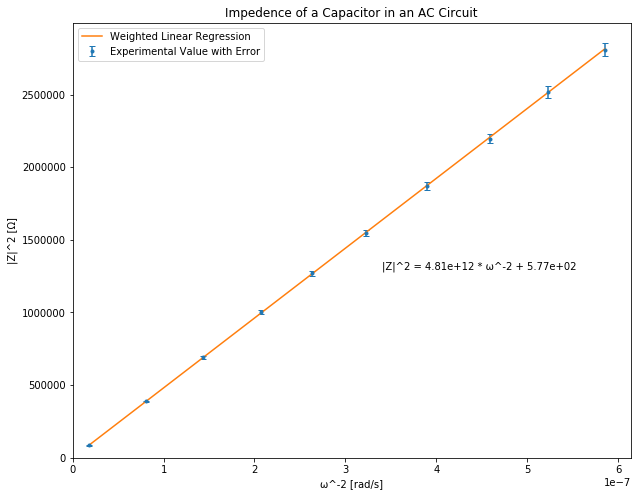
\includegraphics[width=\textwidth]{cap.png}
    \caption{Impedance of an Capacitor in an AC Circuit with Weighted Linear
    Regression where \getMeasuredC}\label{fig:cap}
\end{figure}

\begin{figure}[H]
    \label{fig:par}
    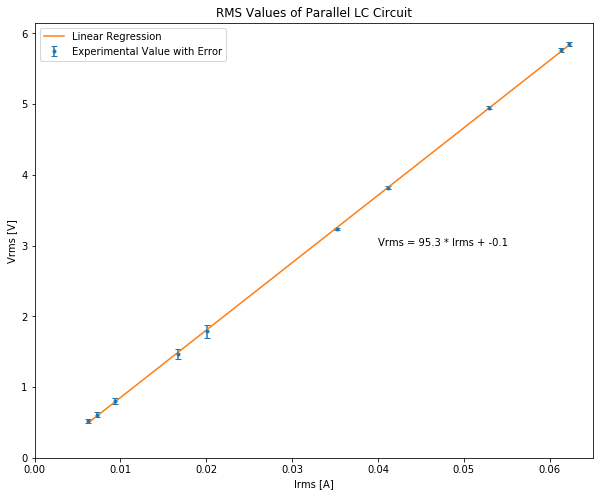
\includegraphics[width=\textwidth]{par.png}
    \caption{RMS Values of Parallel LC Circuit with Linear Regression where
    \getFrequency}

    Note: The input voltage amplitude was varied from the minimum to the maximum
    setting on the function generator.
\end{figure}

\begin{figure}[H]
    \label{fig:ser}
    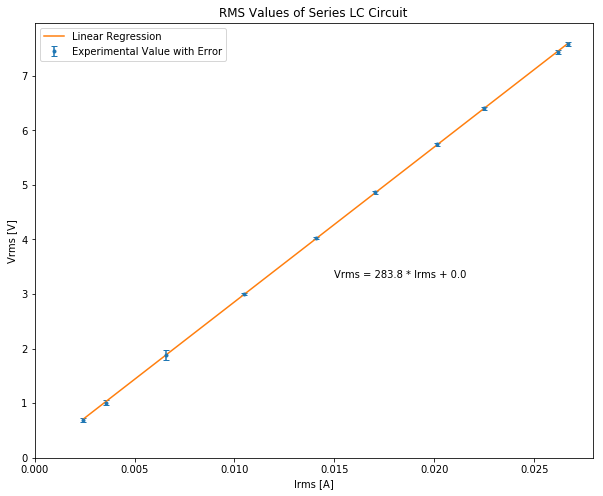
\includegraphics[width=\textwidth]{ser.png}
    \caption{RMS Values of Series LC Circuit with Linear Regression where
    \getFrequency}

    Note: The input voltage amplitude was varied from the minimum to the maximum
    setting on the function generator.
\end{figure}


\section*{Appendix}

\subsection*{Equation List} 
$Z$ is defined as impedance, $V$ is voltage, $I$ is current, $f$ is
Voltage frequency, $L$ is inductance, $C$ is capacitance, and $R$ is resistance.

\begin{equation}
    f = \frac{\omega}{2 \pi}
\end{equation}

\begin{equation} \label{eq1} 
    |Z| = V_{rms}/I_{rms} 
\end{equation}

\begin{equation} \label{eq2} 
    |Z| = R_{L}^2 + \omega^2 L^2
\end{equation}

\begin{equation} \label{eq3}
    |Z| = R_{C}^2 + \frac{1} {\omega^2C^2}
\end{equation}

\begin{equation} \label{eq5}
    Z = R_{L} + j\omega L
\end{equation}

\begin{equation} \label{eq6}
    Z = \frac{1}{j\omega C}
\end{equation}

\begin{equation} \label{eq7}
    Z_{series} = \sum Z_i
\end{equation}

\begin{equation} \label{eq8}
    Z_{parallel}^{-1} = \sum \frac{1}{Z_i}
\end{equation}

\subsection*{Raw Data and Sample Calculations}
Measured values:
\begin{itemize}
    \item \getMeasuredR\
    \item \getMeasuredC\
\end{itemize}

\begin{table}[!htb]
    \caption{Readings and Calculations of AC Circuit with single Inductor with
    measured \getMeasuredR}\label{tab:ind}
    \begin{tabulary}{\textwidth}{CCCCC}
        Frequency[Hz]&Vrms [V] ($\pm$ 0.75\% $\pm$ 2 digits)&Irms [mA] ($\pm$
        0.75\% $\pm$ 2 digits)&Z [$\Omega$]&Error in Z [$\Omega$]\\
        \hline
        200                & 3.02         & 97.2          & 31.07        & 0.16                  \\
        490                & 3.97         & 89.5          & 44.36        & 0.23                  \\
        665                & 4.64         & 85            & 54.59        & 0.27                  \\
        801                & 5.06         & 80.4          & 62.94        & 0.31                  \\
        916                & 5.38         & 76.5          & 70.33        & 0.36                  \\
        1020               & 5.63         & 73.1          & 77.02        & 0.39                  \\
        1114               & 5.83         & 70.1          & 83.17        & 0.42                  \\
        1200               & 6            & 67.5          & 88.89        & 0.45 \\
    \end{tabulary}
\end{table}

\begin{table}
    \caption{Readings and Calculations of AC Circuit with single Capacitor with
    measured \getMeasuredC}\label{tab:cap}
    \begin{tabulary}{\textwidth}{CCCCC}
        Frequency [Hz]&Vrms [V] ($\pm$ 0.75\% $\pm$ 2 digits)&Irms [mA] ($\pm$
        0.75\% $\pm$ 2 digits)&Z [$\Omega$]&Error in Z [$\Omega$]\\
        \hline
        208&7.76&4.63&1.676&0.015\\
        220&7.76&4.89&1.587&0.014\\
        235&7.75&5.23&1.482&0.013\\
        255&7.75&5.67&1.367&0.012\\
        280&7.74&6.22&1.244&0.011\\
        310&7.74&6.87&1.127&0.010\\
        350&7.73&7.72&1.001&0.009\\
        420&7.71&9.28&0.831&0.008\\
        560&7.78&12.48&0.623&0.006\\
        1200&7.69&26.36&0.292&0.001\\
    \end{tabulary}
\end{table}

\begin{table}
    \centering
    \caption{Readings and Calculations of Parallel LC circuit with measured\label{tab:par}
    \getFrequency, \getMeasuredC, \getFrequency}
    \begin{tabulary}{12cm}{CC}
        Vrms [V] ($\pm$ 0.75\% $\pm$ 2 digits) & Irms [mA] ($\pm$ 0.75\% $\pm$ 2 digits)
        \\
        \hline
        0.52&6.27\\
        0.61&7.31\\
        0.8&9.4\\
        1.47&16.73\\
        1.79&20.1\\
        3.23&35.2\\
        3.82&41.2\\
        4.95&52.9\\
        5.76&61.3\\
        5.85&62.2\\
    \end{tabulary}
    \\The input voltage amplitude was varied from the minimum to the maximum
    setting on the function generator. At the maximum setting, the $I_{rms}$ values of the individual component
    were measured as:
    $I_L = 77.2 mA \pm 0.37 mA$
    $I_C = 16.8 mA \pm 0.84 mA $
\end{table}



\begin{table}
    \caption{Readings and Calculations of Series LC circuit with
    measured\label{tab:ser}
    \getFrequency, \getMeasuredC, \getFrequency}
    \centering

    \begin{tabulary}{12cm}{CC}
        Vrms [V] ($\pm$ 0.75\% $\pm$ 2 digits) & Irms [mA] ($\pm$ 0.75\% $\pm$ 2 digits)
        \\
        \hline
        0.69&2.44\\
        1.01&3.55\\
        1.88&6.58\\
        3&10.5\\
        4.03&14.1\\
        4.86&17.03\\
        5.74&20.15\\
        6.4&22.5\\
        7.44&26.2\\
        7.58&26.7\\
    \end{tabulary}
    \\The input voltage amplitude was varied from the minimum to the maximum
    setting on the function generator. At the maximum setting, the $V_{rms}$ values of the individual component were measured as:
    $V_L = 1.89 V \pm 0.94 V$
    $V_C = 9.36 V \pm 0.47 V$
\end{table}

\end{document}
